Há poucos anos que a Computação em Nuvem deixou de ser um tema exclusivo de acadêmicos, hoje se faz presente na vida de pessoas e empresas e muitas vezes passando despercebida em suas rotinas e atividades do cotidiano. Estabelecendo-se como uma importante e fundamental meio computacional. 

A Computação em Nuvem, é de fato um serviço em ebulição e que tem se tornando um paradigma cada vez mais reconhecido e utilizado. Inúmeras empresas têm apoiado e incentivado o uso e o desenvolvimento tão quanto o meio científico. Atualmente, os exemplos do paradigma de computação em nuvem possuem diversas opções para armazenamento ou processamento de dados na nuvem, como a \textit{\sigla{S3}{Simple Storage Service}} da Amazon, Bigtable do Google, ou PNUTS do Yahoo \cite{Binnig2009}. \citeonline{vazquez2014} exemplificam com o crescimento do Instagram, que construíram a sua base de usuários, de mais de 150 milhões de usuários, em menos de quatro anos usando soluções em nuvem.

O aumento da popularidade da computação em nuvem é impulsionado pelas vantagens oferecidas pelo modelo dinamicamente escalável e o rápido desenvolvimento nos últimos anos levou a uma enorme quantidade de publicações. Embora ainda novo, o grande interesse no meio acadêmico e da indústria têm levado a uma quantidade considerável de publicações de artigos científicos nos últimos anos \cite{Heilig2014}.

Como apresentado nos trabalhos de \citeonline{Heilig2014} e \citeonline{Yang2012}, o número de pesquisas têm concentrado esforços na resolução de problemas que em geral envolvem performance e/ou garantia de requisitos de Qualidade de serviço (\textit{\sigla{QoS}{Quality of service}}). 

A computação em nuvem tem emergido como um paradigma flexível de modo a facilitar a gestão de seus recursos e implementar aplicações elásticas em escala sem precedentes \cite{Cervino2012}. Existe uma grande preocupação por parte dos provedores de computação em garantir QoS de uma forma eficiente. Em termos de recursos, significa que os recursos virtuais (\textit{\sigla{VMs}{Virtual Machines}}) e/ou físicos tem devem ser alocados de forma autônoma, para que possam responder às influências externas, como a carga de trabalho. Em geral, os \textit{data center} são muitas vezes subutilizados devido ao excesso de provisionamento, bem como demandas de recursos que variam no tempo de acordo com os sistemas \cite{Padala2007}. \citeonline{Inomata2011} afirma que tempo e dinheiro são investido para projetar, construir, configurar, monitorar e manter recursos computacionais e que o futuro da computação em nuvem é o auto gerenciamento e a atribuição de recursos automáticos aos seus consumidores com base na carga de trabalho.

Atualmente, com o advento e crescimento das aplicações intensivas de dados, que lidam com grandes volumes em tempo real, a dinâmica do sistema passa ser perceptível e apreciável, fenômeno não perceptível claramente para os sistemas computacionais. Na prática, tais aplicações tendem a terem cargas de trabalho variante no tempo, causando inúmeros problemas imprevisíveis no sistema. A computação em nuvem oferece uma infraestrutura elástica ou escalável que pode ser utilizada para obter recursos \textit{on-demand}, no entanto, um problema em aberto é decidir sobre a correta alocação de recursos ao implantar na nuvem \cite{Cervino2012}. De modo geral, um sistema dinâmico não apresenta os efeitos das ações da carga de forma imediata. Como, por exemplo, a velocidade de um carro não muda imediatamente quando o pedal do acelerador é acionado e tão quanto menos uma temperatura em uma sala muda instantaneamente quando um aquecedor é ligado. Da mesma forma que uma dor de cabeça não desaparece logo após tomar uma aspirina, para todos os casos se requer tempo para que o efeito da ação se apresente \cite{Karl2008}.

Este comportamento, dinâmico, começou a pode ser apresentado e apreciado em grande sistemas computacionais, como um súbito aumento de requisições para um \textit{website} onde os servidores não conseguem suportar a demanda. \citeonline{Arlitt2000} apresentam, um trabalho detalhado com os \textit{logs} de requisições do \textit{website} oficial da Copa do Mundo de Futebol do ano de 1998. Os dados foram coletados durante 3 meses e em 30 servidores distribuídos espalhados em 4 pontos do planeta. As requisições superaram a taxa de 1 bilhão, uma média de 11.000 requisições por minuto.

\begin{figure}[htb]
	\centering
	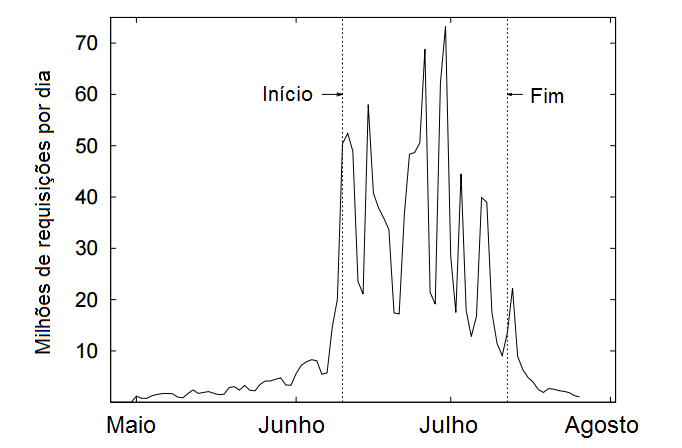
\includegraphics[scale=0.7]{log-world-98.png}
	\caption{Volume diário de tráfego para o Web Site Copa do Mundo}
	\label{fig:log98}		
	\fadaptada{Arlitt2000}
\end{figure}

A Figura \ref{fig:log98} apresenta o volume de requisições diária recebida pelo site Oficial da Copa do Mundo de 1998. No início de Maio até o início do evento (10 de junho) o volume de requisições são baixos em comparação ao início da Copa de 1998. A partir do dia 10 de Junho o volume de requisições cresce enormemente, este fenômeno é chamado de \textit{burstiness} (rajadas). O site de repente tornou-se muito popular devido ao início do evento e permaneceu por um longo período. O dia com maior volume de requisições foi 30 de junho, quando mais de 73 milhões de requisições foram tratadas pelo site, após 30 de junho os volumes de requisições diárias começam a diminuir lentamente até o final da Copa do Mundo, momento em que o volume de tráfego diminui rapidamente \cite{Arlitt2000}.

O \textit{burstiness} no fluxo de requisições são frequentemente encontrados em sistemas cliente-servidor. Esse \textit{burstiness} pode impactar de forma inesperada o desempenho de diferentes mecanismos de alocação de recursos projetados para o gerenciamento de um sistema adaptativo, e, portanto, testar e avaliar esses mecanismos sob cargas de trabalho reproduzíveis e controláveis é fundamental para o projeto do sistema.  Como ilustração, durante o evento promocional de \textit{e-commerce} conhecido como \textit{Black Friday}, na edição de 2012, foi constatado que o tempo de resposta médio aos dias que antecederam 23 de Novembro de 2012, era de 5.3 segundos. A partir das 7 horas do dia evento, observou-se um aumento significativo no tempo de resposta conforme apresentado no gráfico da figura \ref{fig:grafico-black-friday}. Apesar de estar hospedado na \textit{Cloud Computing} e ciente de que o volume de requisições aumentaria, não foi possível manter a qualidade de respostas aos clientes.

Existem muitas abordagens em uso hoje para gerenciar recursos, abrangendo \textit{hardware} e \textit{software}. Ser capaz de medir o desempenho é fundamental para o trabalho da engenharia que busca melhorar as capacidades e a melhor utilização dos recursos.

\begin{figure}[htb]
	\centering
	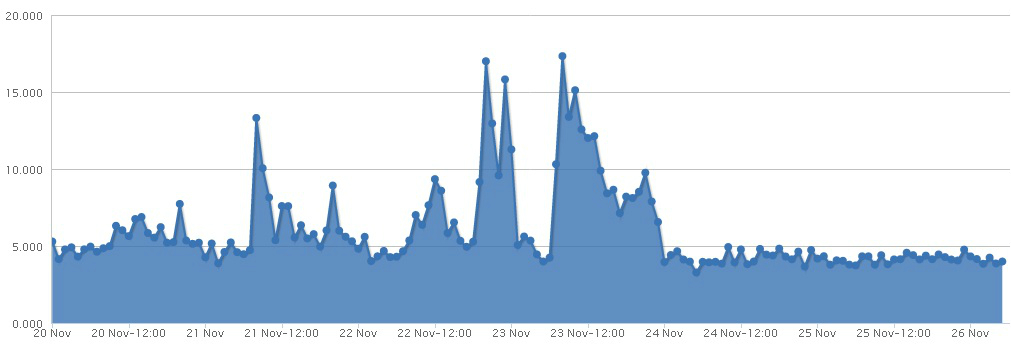
\includegraphics[scale=0.45]{grafico-black-friday.jpg}
	\caption{Tempo de resposta do \textit{Black Friday} Brasil 2012}
	\label{fig:grafico-black-friday}
	\fadaptada{blackfridayNews}
\end{figure}

As técnicas de gerenciamento de recursos são inúmeras, como as de inteligência artificial que utilizam lógica \textit{fuzzy}, algoritmos de mineração de dados e aprendizado de máquina \cite{Nobile2013}. As técnicas de aprendizado de máquina mostram-se interessantes para soluções imediatas, onde não há tempo hábil, inclusive, com abordagens não lineares empregadas para implementar um gerenciador de recursos, responsável pela alteração dinâmica das capacidades computacionais. Outros trabalhos, como o \citeonline{Zhang2007}, buscam identificar padrões de comportamento na carga de trabalho e otimizam a provisão dinâmica de recursos nas máquinas virtuais com base em algoritmos reativos. Utilizando uma abordagem descentralizada e o modelos \textit{Box-Jenkins} de \citeonline{box2011} para particionamento de recursos. \citeonline{Quiroz2009} buscam detectar, por monitoramento, a padronização e a tendência da carga de trabalho com o objetivo de otimizar os recursos. \citeonline{Nobile2013} também propõe o uso de modelos de séries temporais para modelagem de tráfego de tempo real e previsão de demanda, que é usada para criar partições de conexões para diferentes classes de prioridade. Já \citeonline{Zhang2011}, afirma em seu trabalho, que a utilização de cada servidor da nuvem varia de acordo com o tempo de execução, assim a temática de alocação de recurso e o balanceamento da carga de trabalho são desafios para os servidores de computação em nuvem. Logo, \citeonline{Zhang2011}, utiliza de técnicas de estatística e avaliação dos recursos disponíveis para tomar a decisão de qual recurso deve ser alocado.

%Afim de melhor aproveitamentos dos recursos disponíveis em um \textit{data center}, uma das técnicas utilizadas é a teoria de controle, que foi inicialmente proposto em 1960 para lidar com o controle de sistemas lineares invariantes no tempo com parâmetros desconhecidos, que agora alcança o objetivo de circuito fechado satisfatória especificado em termos de engenharia significativos quando a planta incerteza paramétrica é pequena. No entanto, as mudanças nas condições de funcionamento; falha ou degradação do componente; ou mudanças inesperadas na dinâmica do sistema pode tudo a pressuposição de incerteza pequeno, particularmente paramétrico incerteza. Os impactos mencionados acima sempre resultam em respostas de grandes e oscilatórios ou até mesmo instável, quando usando os métodos clássicos de controle adaptativo \cite{Narendra1997}. Essa técnica foi aplicada amplamente em diversas áreas da engenharia, sempre obtendo resultados positivamente satisfatórios e eficientes, até então pouco explorada na computação, os sistemas computacionais não sofriam de variações em seu trabalho, pois as variações nas aplicações eram praticamente imperceptíveis.
%Entretanto, essa técnica, teoria de controle, é pouco explorada e difundida nas áreas da computação mesmo não sendo recente e tento grandes sucessos em outra áreas. Esta técnica apresentar grande potencial de solução para diversos problemas em sistemas computacionais, como o problema de contenção na camada de enlace de dados para redes sem fio \cite{wang2008, boggia2007}.
%Não é de hoje que a teoria de controle tem sido muito bem aplicada e tendo resultados importantíssimos em diversas áreas da engenharia, sendo empregada como uma importante ferramenta na resolução de diversos problemas \cite{Ogata2001}. A evolução da Teoria de Controle na engenharia permitiu desenvolver uma gama de ferramentas de linguagem matemática que auxiliam na descrição de sistemas dinâmicos, como a resposta de diferentes estímulos. Apesar da presença da Teoria de Controle nas diversas áreas da engenharia, em sistemas computacionais é uma área a ser explorada e pesquisada na computação, e que tem ganhado cada vez mais espaço e atenção na área. Pesquisas recentes têm mostrado as possíveis aplicações da Teoria de Controle em sistemas computacionais de auto gerenciamento de recursos \cite{Nobile2013}. Como mostrado por \cite{Abdelzaher2008}, no gerenciamento de memória do IBM DB2, que gerencia a alocação de memória em tempo real, para resolver à variação da carga de trabalho, minimizando o tempo de resposta do sistema foi muito bem utilizada.

\citeonline{Dong2014} afirmam que atualmente, a maioria das aplicações Web são concebidas com sistemas \textit{mult-tiers} (multi-camadas), devido à flexibilidade de escalabilidade, o planejamento de capacidade é um método clássico para determinar a quantidade de recursos exigido para um determinado QoS. No entanto, o planejamento de capacidade é basicamente uma decisão de longo prazo e quase estático, e os recursos são determinados pela taxa de utilização máxima da aplicação para evitar a pena excessiva de QoS.

\citeonline{Lourenco2015} afirma que a partir de um planejamento de capacidade, a gestão de recursos em tempo real, aumenta a sofisticação da arquitetura da solução nos diversos níveis e complexidade, as abordagens convencionais para análise de sistemas computacionais modernos; e concluí que as dinâmicas emergentes das interligações desses sistemas \textit{mult-tiers} pode produzir efeitos transitórios sobre o desempenho, como resposta temporal, ou o amortecimento e/ou comportamento oscilatório. Uma vez que estes efeitos variáveis no tempo podem potencialmente afetar a capacidade de resposta, eficiência e até mesmo a estabilidade global, métodos e ferramentas para avaliação das propriedades dinâmicas de sistemas computacionais são de importância prática para fins da engenharia.

Outra técnica utilizada é a teoria de controle, que foi proposta em 1960 para lidar com o controle de sistemas lineares invariantes no tempo com parâmetros desconhecidos. Não é de hoje que a teoria de controle tem sido muito bem aplicada e tendo resultados importantíssimos em diversas áreas da engenharia, sendo empregada como uma importante ferramenta na resolução de diversos problemas \cite{Ogata2001}. A evolução da teoria de controle na engenharia permitiu desenvolver uma gama de ferramentas de linguagem matemática que auxiliam na descrição de sistemas dinâmicos, como a resposta de diferentes estímulos. Apesar da presença da teoria de controle nas diversas áreas da engenharia, em sistemas computacionais é uma área a ser explorada e pesquisada na computação, e que tem ganhado cada vez mais espaço e atenção na área. Pesquisas recentes têm mostrado as possíveis aplicações da técnica em sistemas computacionais de auto gerenciamento de recursos \cite{Nobile2013}. Como mostrado por \citeonline{Abdelzaher2008}, que estudou e aplicou uma abordagem controle de \textit{feedback} no contexto do gerenciamento de memória do \sigla{DB2}{\textit{Database Management System}} da IBM,  para gerenciar a alocação de memória em tempo real e responder a uma variação da carga de trabalho e minimizar o tempo de resposta do sistema.

Para facilitar o entendimento e lidar com sistemas grandes e complexos, é interessante ter maneiras de validar esses sistemas de modo a garantir o desempenho sem prejudica o QoS. O desempenho de um sistema computacional pode ser medido por meio de técnicas de avaliação de desempenho, sendo assim, existem duas possibilidades básicas de abordagem: modelagem e aferição \cite{Jain1991}.

A teoria de controle utiliza da modelagem, um modelo que é uma representação matemática de um sistema físico, biológico ou de informação, esses modelos nos permitem raciocinar sobre um sistema e fazer previsões sobre como ele se comportará \cite{Karl2008}. Este trabalho está interessado principalmente em modelos de sistemas dinâmicos que descrevem o comportamento de sistemas de entrada e saída. De modo geral um sistema dinâmico não apresenta os efeitos das ações imediatamente quando ocorrem. %Como por exemplo, a velocidade de um carro não muda imediatamente quando o pedal do acelerador é acionado e tanto quanto menos uma temperatura em uma sala muda instantaneamente quando um aquecedor é ligado. Da mesma forma, que uma dor de cabeça não desaparece logo após tomar uma aspirina, para todos os casos se requer tempo para que o efeito da ação se apresente \cite{Karl2008}.

Há caso em que existe o interesse em controlar a dinâmica deste sistema, para tanto é necessário modelar o sistema em questão e projetar um controlador que manipulará a sua dinâmica. Para trabalhar com estes sistemas deve-se ser capaz de modelar um sistema dinâmico, que em termos matemáticos é extrair um modelo matemático e analisar suas características dinâmicas. Um modelo matemático de um sistema dinâmico é definido como um conjunto de equações que representa a dinâmica do de maneira relativamente razoável. Percebe-se que um modelo matemático não é exclusivo para um determinado sistema. Um sistema pode ser representando de muitas maneiras diferentes e, por conseguinte, podem ter diversos modelos matemáticos, dependendo da perspectiva, uns mais precisos que outros, e outros mais simplificados \cite{Ogata2001}.

Em geral, é possível representar sistemas dinâmicos através de equações diferenciais obtidas com base nas leis básicas da Física. Esses sistemas de equações diferenciais descrevem uma determinada dinâmica do sistema no domínio do tempo e, com o desenvolvimento dessas equações, é possível identificar propriedades fundamentais do sistema \cite{Nobile2013}.


A avaliação por aferição, medição direta via instrumentação apropriada, adequa-se muito bem as necessidade, no entanto, é necessário a existência e disponibilidade do sistema ou protótipo, pois a avaliação é feita através de estímulos às entradas (\textit{benchmark}) e leitura de suas saídas, possibilitando testes de caixa preta onde não é exigido conhecimento sobre o funcionamento interno do sistema, possibilitando a aquisição de resultados precisos devido à aplicação em sistema real \cite{Nobile2013}, como em um sistema dinâmico, no qual o comportamento do sistema evolui com o tempo, em resposta a estímulos externos.

Independente da abordagem, aferição ou modelagem, o importante da técnica de avaliação utilizada é a abrangência mediante ao comportamento em condição estática e dinâmica do sistema \cite{helder2014}.


\section{Motivação}

Embora amplamente aplicada e difundida em diversas áreas da engenharia e ciência, a avaliação de desempenho em regime transitório é pouco explorada e usada em sistemas computacionais, possivelmente está relacionado habituais e tradicionais sistemas computacionais, onde não é possível perceber a dinâmica do mesmo. Aplicativos móveis, \textit{notebooks} e \textit{\sigla{PCs}{Personal Computers}} estão criando cada vez maior capacidade computacional, que estimulam os sistemas enriquecidos de serviços, como entretenimento de mídia e redes sociais, jogos, etc. Emergindo e apresentando a dinâmica do sistema e despertando o interesse na análise transiente em sistemas computacionais, que ocorre concomitantemente ao aparecimento de aplicações, assim como os sistemas mecânicos ou elétricos que apresentam propriedades de inercia na transformação de estímulos (entrada) em resposta (saída) onde a dinâmica dos mecanismos constituintes se torna não negligenciável. É o caso de sistemas distribuídos de larga escala, de grande complexidade e envolvendo a interação pervasiva com sistemas físicos \cite{Egami2011, Kannan2011}. 

Neste contexto de pesquisa, o \textit{\sigla{LaSDPC}{Laboratório de Sistemas Distribuídos e Programação Concorrente}}\footnote{\url{http://www.lasdpc.icmc.usp.br}}, onde desenvolve este projeto, trabalhos anteriores lidam com essa temática, como o trabalho de \citeonline{Nobile2013}, que apresentou resultados que valorizam e apreciam os impactos no desempenho de um sistema com características dinâmicas, hospedado em um ambiente de computação em nuvem de recursos elásticos e com mecanismos de provisão de QoS, através da modelagem das propriedades de resposta transiente do sistema que são aplicadas e gerenciadas com  técnicas de teoria de controle. Em outro trabalho, \citeonline{Lourenco2015} apresentou uma especificação de uma arquitetura conceitual que separa responsabilidades de simulação dinâmica em um conjunto de preocupações básicas, e formaliza um modelo de referência abstrata para a concepção de ferramentas de simulação. Junto a instância da classes abstratas e implementadas algumas políticas de controle básicos e com o modelo podem ser facilmente utilizados em experimentos de simulação com o CloudSim. O trabalho de \citeonline{Edwin2015}, em desenvolvimento no LaSDPC, estuda e define uma metodologia de análise transiente dedicado a sistemas computacionais dinâmicos reais utilizando da especificação arquitetural de \citeonline{Lourenco2015}. A principal contribuição pretendida é a formulação e definição de uma metodologia para seu emprego em sistemas, cuja a metodologia deverá ser capaz de descrever e especificar os passos para modelar o sistema, projetar um controlador e analisar os resultados transiente mediante as variações na carga de trabalho. Para tanto, o trabalho de \citeonline{Edwin2015} utiliza de um \textit{benchmark} para a validação experimental de sua metodologia. No entanto, o \textit{benchmark} escolhido por \citeonline{Edwin2015} não contempla das especificações apresentadas por \citeonline{Lourenco2015}.

Segundo \citeonline{Binnig2009} os \textit{benchmarks} tradicionais não são suficientes para a análise desses novos serviços de elasticidade da nuvem. O principal desafio dos novos \textit{benchmarks} é fazer com que os resultados apresentados, ou seja as métricas, ofereçam informações relevantes a esses diferentes serviços e com diferentes capacidades e garantias desses serviços. \citeonline{Dong2014} afirmam que, a maioria das aplicações Web são concebidas como sistemas \textit{mult-tiers}, devido à flexibilidade e capacidade de reutilização de software, porem é difícil de modelar o comportamento de aplicações Web de várias camadas, devido ao fato de que a carga de trabalho estimula a dinâmica do sistema nos diferentes níveis da camada.

No âmbito da análise de desempenho em sistemas computacionais, definimos o \textit{benchmarking} como o ato de medir e avaliar o desempenho computacional, protocolos de rede, dispositivos e redes, sob condições de referência, em relação a uma avaliação de referência. O objetivo deste processo de \textit{benchmarking} é permitir a comparação equitativa por diferentes soluções, ou entre desenvolvimentos subsequentes de um \textit{\sigla{SUT}{\textit{System Under Test}}}. \textit{Benchmarking} é o principal método para medir o desempenho de uma máquina ou sistema. O \textit{benchmarking} refere-se à execução de um conjunto de programas representativos em diferentes computadores e redes, medindo os resultados. Esses resultados são utilizados para avaliar o desempenho de um determinado sistema com uma carga de trabalho bem definida \cite{Menasce2001}.

Entretanto, não existe aparato ferramental para a exploração dessas técnicas, apesar de existir diversos \textit{benchmarks} e ferramentas para o estudo, nenhuma delas estimulam a dinâmica transiente do sistema e permitem uma avaliação em regime transiente, que se faz necessário para a pesquisa. A proposta deste trabalho é identificar um \textit{benchmark} e adequá-lo de maneira em que estimule a dinâmica do sistema possibilitando uma avaliação transiente.


\section{Objetivo}
Este trabalho tem por objetivo a extensão de um \textit{framework} do \textit{benchmark} Bench4Q afim de atender os requisitos do modelo \textit{\sigla{MEDC}{\textit{Monitor, Effector, Demanda and Capacity}}}, proposto por \citeonline{Lourenco2015}. O objetivo restringe ao modulo de modulação da carga de trabalho, gerado pelo \textit{benchmark}, acrescendo-o de provisões nativas para gerar perturbações capazes de excitar e produzir o regime transiente do sistema SUT do \textit{benchmark}, onde poderá ser apreciado a sua dinâmica. A contribuição almejada é a disponibilização de um \textit{benchmark} que auxilie a análise de sistemas dinâmico e que possibilite a analise transiente do mesmo. São consideradas perturbações configuráveis na carga de trabalho, e resultados são apresentados pelo \textit{benchmark}.


